%====================================================================
%====================================================================
\section{Problem 2: Network structure}
\frame{\frametitle{Outline} \tableofcontents[currentsection]}
%====================================================================
\subsection{Network structure}
%====================================================================
\frame{\frametitle{Understanding the network structure} 

  \paragraph{Tree species interactions \refer{VPD08}.} $n = 51$ tree species, $d =3$ covariates
  \begin{itemize}
    \item $x_{ij} =$ vector of similarities (taxonomic, geographic, genetic) between species $i$ and $j$
    \item $Y_{ij} =$ number of fungal parasites shared by species $i$ and $j$
  \end{itemize}
  
  \bigskip \bigskip \pause
  \paragraph{Random graph model.}
  $$
  \Gcal = Y = [Y_{ij}]_{1 \leq i, j \leq n} \sim \Fcal(X, \theta, Z)
  $$
  \begin{itemize}
    \item $\theta =$ model parameters
    \item $Z =$ species role
  \end{itemize}
  
  \bigskip \bigskip \pause
  \paragraph{More precisely.} Given the covariates $X$, the model parameters $\theta$ and the species roles $Z$, be able to evaluate
  $$
  \Pr\left\{Y_{11} = 17 \text{ and } Y_{12} = 12 \text{ and } 
  Y_{23} = 10 \text{ and } Y_{45} = 5 \text{ and } \dots\right\}
  $$
  
}
  
%====================================================================
\frame{\frametitle{Network model} 

  \bigskip
  \paragraph{Problem 2.} Decipher species roles in the observed network

  \bigskip \bigskip \pause
  \paragraph{Stochastic block model (SBM, \refer{HoL79}).} Under species roles in the observed network
  \begin{itemize}
    \item $K$ clusters (roles)
    \item each species $i = 1 \dots n$ belongs to one (\emphase{unobserved}) cluster
    \item the distribution of the interaction $Y_{ij}$ depends on the cluster memberships $Z_i$ and $Z_j$.
  \end{itemize}
  
  \bigskip \bigskip \pause
  \paragraph{Tree species interactions.} 
  \begin{tabular}{ccc}
    \hspace{-.04\textwidth}
    \begin{tabular}{p{.35\textwidth}}
      \multicolumn{1}{c}{Observed interactions} \\
      \footnotesize{
      \begin{tabular}{c|rrrrr}
            & sp1 & sp2 & sp3 & sp4 & \dots \\
        \hline
        sp1 &  17 &  12 &   9 &   3 & \\
        sp2 &  12 &  16 &  10 &   3 & \\
        sp3 &   9 &  10 &  11 &   1 & \\
        sp4 &   3 &   3 &   1 &  23 & \\
        sp5 &   2 &   1 &   1 &   5 & \\
        \vdots & 
      \end{tabular}}
      \\ ~\\ ~\\ 
    \end{tabular}
    &
    \begin{tabular}{p{.25\textwidth}}
      \multicolumn{1}{c}{Adjacency matrix} \\
      \includegraphics[height=.25\textwidth, trim=0 0 0 50, clip=]{\fignet/Tree-adjMat}
    \end{tabular}
    &
    \begin{tabular}{p{.25\textwidth}}
      \multicolumn{1}{c}{Clustered matrix} \\
      \includegraphics[height=.25\textwidth, trim=0 0 0 50, clip=]{\fignet/Tree-adjMat-SBMnull}
    \end{tabular}
  \end{tabular}

}

%====================================================================
\subsection{Stochastic block-model}
%====================================================================
\frame{\frametitle{Tree species interaction network} 

  \bigskip
  \paragraph{Poisson SBM \refer{MRV10}.} Interactions = counts:
  \begin{itemize}
    \item each species belongs to cluster $k$ with probability $\pi_k$ ($1\leq k \leq K$)
    $$
    \Pr\{Z_i = k\} = \pi_k
    $$
    \item if species $i$ belongs to cluster $k$ and species $j$ to cluster $\ell$, the number of shared parasites has a Poisson distribution with parameter $\lambda_{k\ell}$:
    $$
    (Y_{ij} \mid Z_i = k, Z_j = \ell)\sim \Pcal(\lambda_{k\ell})
    $$
  \end{itemize}

  \bigskip \pause
  \paragraph{Model without covariates.} $\widehat{K} = 7$ clusters \\ ~\\ 
  \begin{tabular}{ccc}
    Adjacency matrix & Clustered matrix & Clade composition \\
    \includegraphics[height=.25\textwidth, trim=0 0 0 50, clip=]{\fignet/Tree-adjMat} &
    \includegraphics[height=.25\textwidth, trim=0 0 0 50, clip=]{\fignet/Tree-adjMat-SBMnull}
    &
    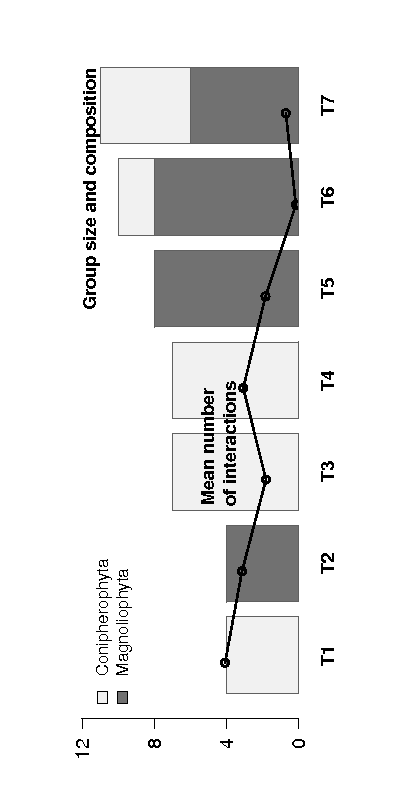
\includegraphics[height=.2\textwidth, width=.3\textwidth, trim=150 200 150 200, clip=]{\fignet/MRV10_AoAS_Q7_group}
  \end{tabular}
  
}

%====================================================================
\frame{\frametitle{Accounting for covariates} 

  \bigskip
  \paragraph{Poisson SBM with covariates.} 
  \begin{itemize}
    \item $x_{ij} =$ \emphase{taxonomic distance} between species $i$ and $j$
    \item if species $i$ belongs to cluster $k$ and species $j$ to cluster $\ell$, the number of shared parasites has a Poisson distribution with parameter $\lambda_{k\ell}$:
    $$
    (Y_{ij} \mid Z_i = k, Z_j = \ell)\sim \Pcal(e^{\alpha_{k\ell} + \beta x_{ij}})
    $$
  \end{itemize}

  \bigskip \pause
  \paragraph{Model with covariates.}  $\widehat{K} = 4$ clusters, $\widehat{\beta} = - .317$ \\ ~\\
  \begin{tabular}{ccc}
    Adjacency matrix & Clustered matrix & Clade composition \\
    \includegraphics[height=.25\textwidth, trim=0 0 0 50, clip=]{\fignet/Tree-adjMat} &
    \includegraphics[height=.25\textwidth, trim=0 0 0 50, clip=]{\fignet/Tree-adjMat-SBMtaxo}
    &
    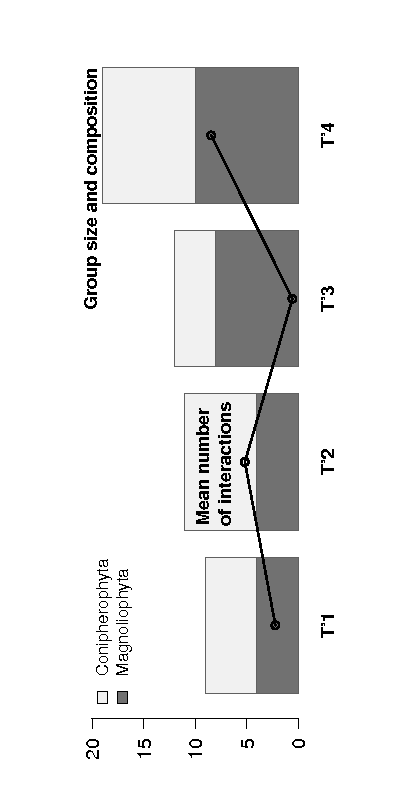
\includegraphics[height=.2\textwidth, width=.3\textwidth, trim=150 200 150 200, clip=]{\fignet/MRV10_AoAS_Q4_group}
  \end{tabular}
  
}

